\usepackage{caption}
\usepackage{subcaption}

\section{Validierung}
Im folgenden Abschnitt wird die Validierung beschrieben. Die Validierung dient zum Auffinden und Beheben von Fehlern, um so eine korrekte Funktion des Programms garantieren zu können. Zum einen wurden die Berechnungen und Simulationen von Matlab überprüft, zum anderen die Software, aufgeteilt in die Teilbereiche Benutzeroberfläche und Berechnungen.

\subsection{Matlab}

\subsubsection{Programmierung}
%Problem/Fragestellung:
%- Wie kann die korrekte Funktion der Matlab-Programme überprüft werden?
%Lösung: Die berechneten Antworten werden mit den Antworten von Herrn Niklaus verglichen.
Die Berechnung der Regler wurde zuerst mittels m-Files in Matlab implementiert. Zur Überprüfung der von Matlab gelieferten Werte wurden diese mit den Werten vom Fachcoach Peter Niklaus verglichen.


\subsubsection{Simulation}
%Problem/Fragestellung:
%- Wie kann die Matlab-Simulation überprüft werden?
%Lösung: Sie wird mit Simulink überprüft.
Mittels Simulink wurde der geschlossene Regelkreis simuliert.

\subsection{Java Software}

\subsubsection{Benutzeroberfläche}
%Problem/Fragestellung:
%- Wie können Probleme oder Konflikte bei der Benutzeroberfläche ausgeschlossen werden?
%Mehrere unabhängige User testen die Software.

%Um die einfache Handhabung der Software zu überprüfen wurde die Software im ganzen Projektteam sowie von mehreren unabhängigen Benutzern getestet. Die so gefundenen Unklarheiten oder Probleme wurden behoben.

\subsubsection{Model}
%Problem/Fragestellung:
%- Wie wird die korrekte Funktion der Software überprüft?
%Lösung: Die Software mit mit JUnit getestet, wobei die Resultate von Matlab erwartet werden.
Die Plausibilität der Schrittantworten konnte relativ einfach optisch mit den Graphen überprüft werden, da das Verhalten der einzelnen Regler bekannt ist. Zur genauen Überprüfung der einzelnen Klassen wurden sämtliche Klassen des Models mittels JUnit mit den Ergebnissen von Matlab verglichen.

\subsubsection{Performancevergleich Partialbruchzerlegung und IFFT}\label{residuenvsifft}
Es wurde festgestellt dass das Berechnen des Schrittantwortes mittels IFFT-Methode merkbar langsam ist - vorallem dann, als das iterative Approximieren des Überschwingens implementiert wurde, was dazu führte, dass die Schrittantwortberechnung mehrmals ausgeführt werden musste.

Durch Reduzieren der Anzahl Pünkte kann die Berechnung beschleunigt werden, jedoch kommt dies auf Kosten von Genauigkeit.

\begin{figure}
\centering
\begin{subfigure}{.33\textwidth}
	\centering
	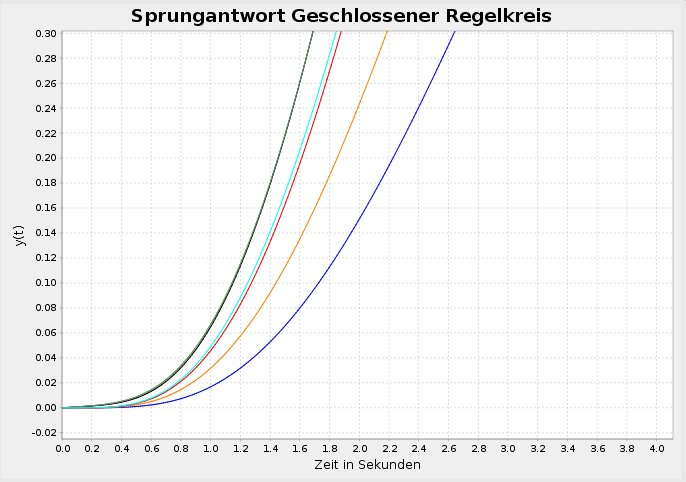
\includegraphics[width=.4\linewidth]{./ifft_4096.jpg}
	\caption{A subfigure}
	\label{fig:sub1}
\end{subfigure}
\begin{subfigure}{.33\textwidth}
	\centering
	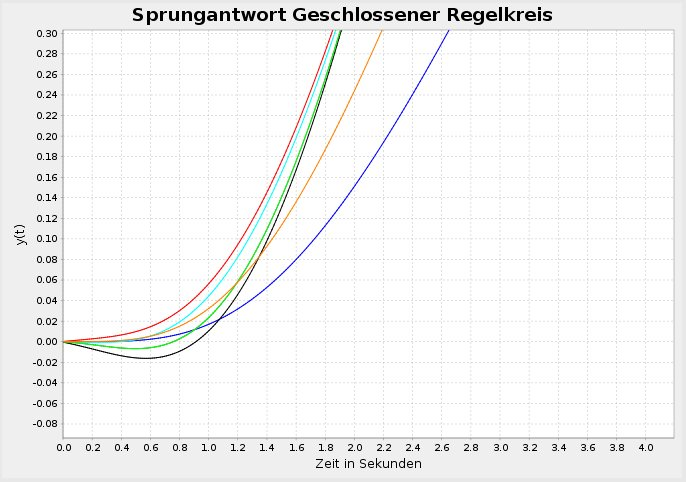
\includegraphics[width=.4\linewidth]{./ifft_2048.jpg}
	\caption{A subfigure}
	\label{fig:sub2}
\end{subfigure}
\begin{subfigure}{.33\textwidth}
	\centering
	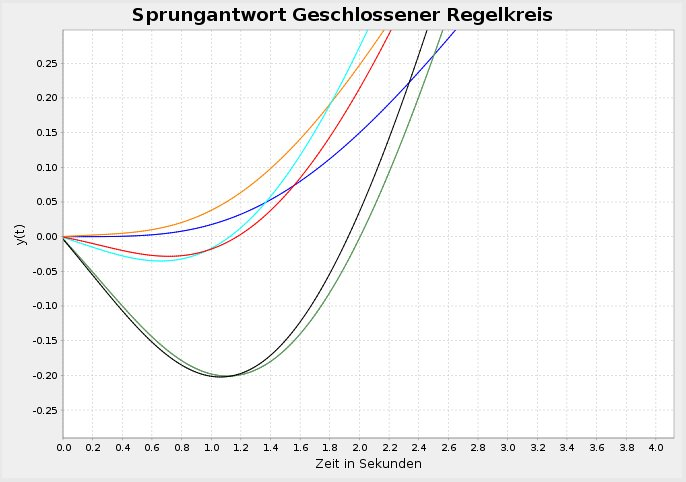
\includegraphics[width=.4\linewidth]{./ifft_1024.jpg}
	\caption{A subfigure}
\caption{A figure with three subfigures}
\label{fig:test}
\end{figure}

Es wurde entschieden, eine alternative Berechnungsmethode zu implementieren: Schrittantwortberechnung mittels Partialbruchzerlegung.

